% para agregar la carpeta de las imagenes
%\graphicspath{{./nombre de la carpeta/}}

%el codigo principal solo contiene el tipo de documento, la caratula y la forma de llamar a los otros archivos, asi como imprimir bibilografia y el indice.

\documentclass[11pt,a4paper]{article}
% Configuración de la codificación de entrada
\usepackage[utf8]{inputenc}

% Configuración de la codificación de salida
\usepackage[T1]{fontenc}

% Paquete para el idioma y comillas
\usepackage[spanish,es-tabla]{babel}
\usepackage{csquotes}

\usepackage{hyphenat}
\usepackage{microtype}

\hyphenation{ex-am-ple hy-phen-a-tion}
\hyphenpenalty=500
\tolerance=1000

% Tamaño de la página (A4) y márgenes
\usepackage[a4paper,top=2cm,bottom=2cm,left=3cm,right=3cm,marginparwidth=1.75cm]{geometry}

% Otros packages
\usepackage{amsmath}
\usepackage{graphicx}
\usepackage[colorlinks=true, allcolors=blue]{hyperref}
\usepackage[utf8]{inputenc}

\usepackage{hyperref}
\usepackage{amsmath}
\usepackage[usenames]{color}
\usepackage{amsfonts}
\usepackage{amssymb}
\usepackage{graphicx}
\usepackage{caption}
\usepackage{enumerate} 
\usepackage{siunitx}
\usepackage{upgreek}
\usepackage{epsfig}
\usepackage{multirow}
\usepackage{colortbl}
\usepackage{xspace}    

% para las tablas
\usepackage{multicol,multirow, array} 
\usepackage[table,xcdraw]{xcolor}
\usepackage[table]{xcolor}
\captionsetup{justification=centerlast,labelfont=bf,font=sf}
\usepackage{subfigure}
\usepackage[T1]{fontenc}
\usepackage{fourier}
\usepackage{fancyhdr}
\usepackage{float} 
\usepackage{steinmetz}
\setcounter{equation}{0}
\usepackage{biblatex} %llama al archivo donde estan todas las librerias include


%%encabezado
\rhead{\begin{picture}(0,0)	\put(-22,0) {
\includegraphics[height=1cm]{caratula/logounsl.png}} \end{picture}}
\lhead{\begin{picture}(0,0)	\put(0,0) {
\includegraphics[height=1cm]{caratula/logo_depto.jpg}} \end{picture}}
\chead{\vspace{-.05cm}\textcolor{gray}{Sistemas de Comunicaciones, teoría de la información y Análisis de Señales - TP N.$^o$1} \vspace{.25cm}}

%%
%pie de pagina
\rfoot{\textcolor{gray}{Comunicaciones I - 2025}}
\lfoot{\textcolor{gray}{Marcos Lucero - Nahuel Ramires - Agustín Cappiello}}
\cfoot{\textcolor{gray}{\thepage}}  % Cambiar el número de página a gris



\begin{document}
    %caratula
    \begin{titlepage}	  
    		\centering
    		
    		% --- Logo UNSL ---		
    		\begin{figure}
    			\centering
    			
\includegraphics[width=0.15\linewidth]{caratula/logo-unsl.jpg}
    		\end{figure}     
    		
    		% --- Datos de la asignatura ---
    		{\scshape\LARGE Universidad Nacional de San Luis\\}
    		{\scshape Facultad de Ciencias Físico Matemáticas y Naturales\par}
    		{\scshape Ingeniería Electrónica con O.S.D.\par}
    		\vspace{2cm} 
    		
    		\Large \textbf {Asignatura:\\} 
    		\bigskip
    		\LARGE {\Huge Comunicaciones I}
    		\vspace{0.3cm}
    		
    		% --- Datos del informe / TP ---
    		\LARGE \textbf {Trabajo Practico N° 2\\} 
    		\vspace{0.7cm}
    		\LARGE \textbf {“Multipath, interferencias, rudio - Señales y Procesos Aleatorios”}

    		\vspace{2cm}
    		% --- Datos del alumno ---  
    		\LARGE \textbf {Estudiantes:\\} 
    		\LARGE Marcos Lucero \\ Nahuel Ramires\\ Agustín Cappiello\\
    		\bigskip
    		
    		
    		\vspace{1cm}
    		
    		% --- Datos de los profesores ---  
    		\Large \textbf {Profesores Responsables:\\} 
    		\bigskip
    		\Large Alejandro Marwan Geraiges Magrini. \\ Roberto Kiessling.
    		
    		
    		\vspace{3cm}
    		
    		% --- Año ---  
    		\Large \textbf {Año:\\} 
    		\Large 2025	
    	\end{titlepage}
    %fin caratula	
    
    \tableofcontents %Para el indice

    \section{Actividad 1}

\subsection*{Una antena transmisora emite una señal cosenoidal \( x(t) = A \cos(2\pi f_t t) \), donde \( A = 17 \, \text{W} \) y \( f_t = 532 \, \text{kHz} \). 
La antena receptora capta dos señales provenientes de dicha antena transmisora. La primera de ellas recorre el camino directo, con una distancia recorrida 
\( D_1 \). Mientras que la segunda, debido a una reflexión en un obstáculo, recorre una distancia \( D_2 \). Ambas señales sufren distintas atenuaciones, se 
suponen que son también aproximadamente cosenoidales y que viajan a la velocidad de la luz en el vacío, no sufriendo ninguna distorsión en su recorrido. Para 
el ejercicio debe considerarse los siguientes valores de atenuación y distancia:}

\begin{align*}
    A_1 &= 10\% & A_2 &= 25\% \\
    D_1 &= 11 \, \text{km} & D_2 &= 14.5 \, \text{km}
\end{align*}

\subsection*{a) Si las señales recibidas se suman en la antena receptora. ¿Cuál es el resultado de esto? Graficar. }

Las señales recibidas se expresan de la siguiente manera:

    \[
        y_1(t) = 0.9 \cdot 17 \cos(2\pi f_1 (t - \tau_1))
        \]
        \[
        y_2(t) = 0.75 \cdot 17 \cos(2\pi f_1 (t - \tau_2))
    \]

donde los retardos temporales son calculados como:

    \[
        \tau_1 = \frac{D_1}{c} = \frac{11000}{3 \times 10^8} = 36.67 \, \mu s
        \]
        \[
        \tau_2 = \frac{D_2}{c} = \frac{14500}{3 \times 10^8} = 48.33 \, \mu s
    \]

La señal resultante es la suma de la señal transmitida por un camino directo y de la señal reflejada \(y(t) = y_1(t) + y_2(t)\) 
\bigskip


\begin{figure}[H]
    \centering
        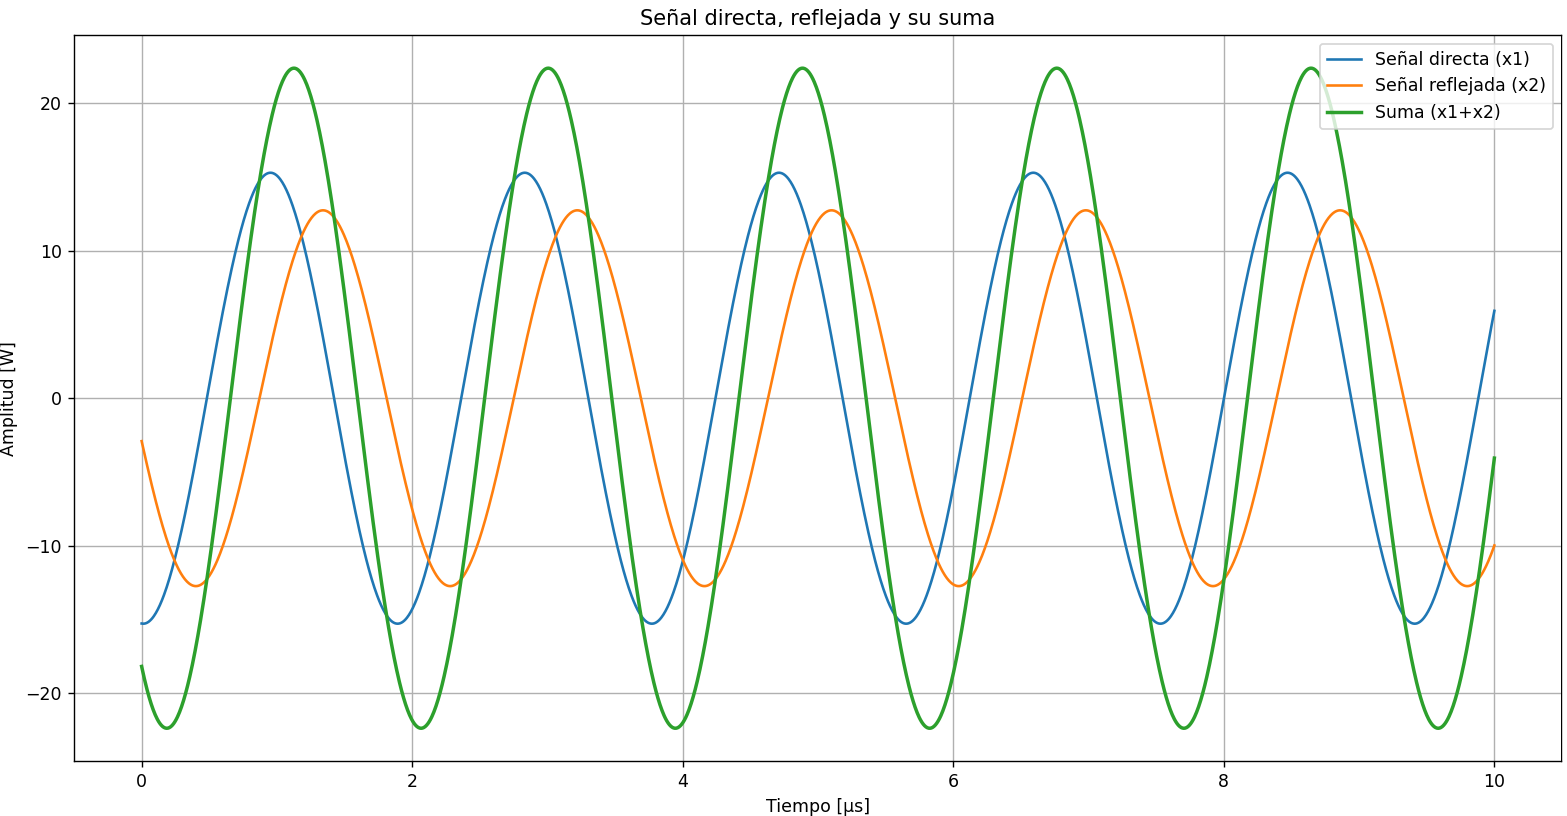
\includegraphics[width=0.8\textwidth]{imagenes/Actividad_1/grafico_532kHz.png}
        \caption{Señal resultante a 532 kHz.}
        \label{fig:532kHz}
    \end{figure}
\bigskip

En la Fig. \ref{fig:532kHz} se observa la señal cosenoidal trasmitida en su camino directo y reflejado, la suma de las dos es la que 
llega a la antena receptora. Como se observa, tienen diferente amplitud y fase debido a las atenuaciones y un retardo temporal por las 
diferentes distancias.
\bigskip

\subsection*{b) Suponer ahora que la frecuencia aumenta a 600 kHz. ¿Qué sucede? Graficar. }

Hay dos trayectorias:
    \[
         D_1 = \SI{11}{km} \qquad D_2 = \SI{14.5}{km}.  
    \]
\bigskip

La diferencia es:
    \[
        \Delta D = D_2 - D_1 = \SI{3.5}{km} = \SI{3500}{m}.
    \]
\bigskip

El retardo entre ambas:
    \[
        \Delta \tau = \frac{\Delta D}{c} = 
        \frac{3500}{3 \cdot 10^{8}}
        \approx 1.1667 \times 10^{-5}\,\text{s}.
    \]

\bigskip

La diferencia de fase entre ellas es:
    \[
        \Delta\varphi = 2\pi f \,\Delta\tau.
    \]


Las dos señales quedan en fase cuando su diferencia de fase es un múltiplo entero de \(2\pi\):
    \[
        \Delta\varphi = 2\pi n,\qquad n=0,1,2,\dots
    \]


    \[
        2\pi f \,\Delta\tau = 2\pi n \quad\Longrightarrow\quad f=\frac{n}{\Delta\tau}.
    \]
\bigskip

Para \(\Delta\tau=1.1667\times10^{-5}\,\text{s}\):
    \[
        f_n=\frac{n}{1.1667\times10^{-5}}.
    \]
\bigskip

Para \(n=7\):
    \[
        f_7=\frac{7}{1.1667\times10^{-5}}=600\,\text{kHz}.
    \]
\bigskip

A \(f=600\,\text{kHz}\) la diferencia de fase es:
    \[
        \Delta\varphi=2\pi f \,\Delta\tau=2\pi\cdot 600000\cdot1.1667\times10^{-5}
        =2\pi\cdot 7=14\pi,
    \]
que es exactamente 7 ciclos completos de diferencia. Por lo tanto, las señales quedan en fase. Por lo tanto, la señal resultante se 
observa en la Fig. \ref{fig:600kHz}.

    \begin{figure}[H]
        \centering
        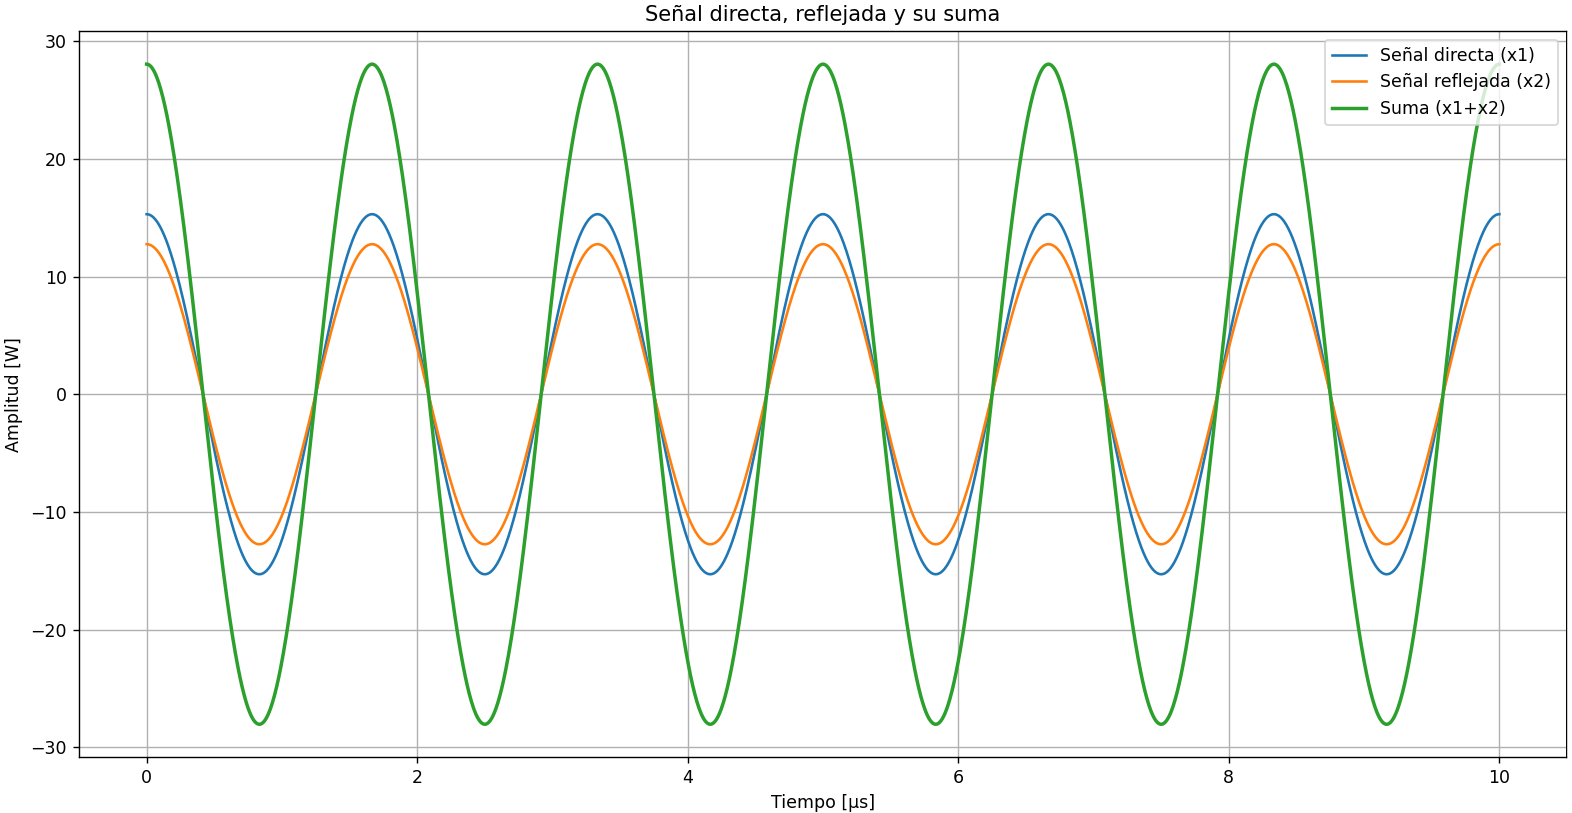
\includegraphics[width=0.8\textwidth]{imagenes/Actividad_1/grafico_600kHz.png}
        \caption{Señal resultante a 600 kHz.}
        \label{fig:600kHz}
    \end{figure}


\subsection*{c) Suponer que las señales sufren la misma atenuación. ¿Existe alguna frecuencia a la cual la señal recibida sea nula? Explicar el concepto.}

Cuando ambas señales sufren la misma atenuación, sus amplitudes se igualan, creando las condiciones ideales para que ocurra \textbf{interferencia destructiva 
total}. Para que la señal recibida sea nula, deben cumplirse dos condiciones fundamentales:

    \begin{enumerate}
        \item \textbf{Iguadad de amplitudes}: $A_1 = A_2$
        \item \textbf{Desfase de 180°}: $\Delta\phi = (2k+1)\pi$ rad, donde $k = 0, 1, 2, \ldots$
    \end{enumerate}

La diferencia de fase entre ambas señales está determinada por la relación:

    \[
        \Delta\phi = 2\pi f \frac{\Delta D}{c}
    \]

Donde:
    \begin{itemize}
        \item $\Delta D = D_2 - D_1 = 3.5 \, \text{km} = 3500 \, \text{m}$
        \item $c = 3 \times 10^8 \, \text{m/s}$
    \end{itemize}

Para obtener cancelación total:

    \[
        2\pi f \frac{\Delta D}{c} = (2k+1)\pi
    \]

Simplificando:

    \[
        2f \frac{\Delta D}{c} = 2k+1
    \]

    \[
        f = \frac{(2k+1)c}{2\Delta D}
    \]
Calculando las primeras tres frecuencias críticas donde se produce cancelación total:
    \begin{itemize}
        \item $k = 0$: $f_0 = \dfrac{3 \times 10^8}{7000} \approx 42.857 \, \text{kHz}$
        \item $k = 1$: $f_1 = \dfrac{3 \cdot 3 \times 10^8}{7000} \approx 128.571 \, \text{kHz}$
        \item $k = 2$: $f_2 = \dfrac{5 \cdot 3 \times 10^8}{7000} \approx 214.286 \, \text{kHz}$
    \end{itemize}

El fenómeno descrito constituye un caso clásico de \textbf{interferencia por multitrayectoria} en sistemas de comunicaciones. Las frecuencias en las que se 
produce cancelación total aparecen equiespaciadas en el dominio frecuencial, formando un patrón periódico cuya periodicidad depende directamente de la 
diferencia de caminos $\Delta D$. Matemáticamente, existe un conjunto infinito y discreto de frecuencias críticas dadas por la expresión:

\[
f_k = \frac{(2k+1)c}{2\Delta D}, \quad k = 0, 1, 2, \ldots
\]

donde $c$ es la velocidad de la luz. Este resultado tiene implicancias directas en el diseño de sistemas de comunicación, donde resulta esencial evitar la 
transmisión en dichas frecuencias críticas o, alternativamente, implementar técnicas de diversidad como el uso de múltiples antenas o saltos en frecuencia 
para mitigar los efectos adversos de la interferencia por multitrayectoria.
 %llama los otros 
	\section{Actividad 2}

En un sistema determinado de comunicaciones, en el que una señal sinusoidal 
\(x(t)=A\sin(2\pi f t)\) pasa a través de un filtro lineal de fase no constante. 
La respuesta en frecuencia del filtro es 
\(H(f)=|H(f)|\,e^{j\beta(f)}\), 
donde \(\beta(f)=-\alpha f\) es la fase dependiente de la frecuencia.

\[
\tau_{p}=\frac{\beta(f)}{2\pi f}
\qquad
\tau_{g}=-\frac{1}{2\pi}\frac{d\beta(f)}{df}
\]


\noindent a) Calcular el retardo de fase y retardo de grupo.
\bigskip

\[
\tau_p = \frac{\beta(f)}{2\pi f}
       = \frac{-\alpha f}{2\pi f}
       = -\frac{\alpha}{2\pi}
\]

\[
\tau_g=-\frac{1}{2\pi}\frac{d\beta}{df}
      =-\frac{1}{2\pi}(-\alpha)
      =\frac{\alpha}{2\pi}
\]
\bigskip

\noindent b) ¿El retardo de fase y el retardo de grupo es constante o depende de la frecuencia?
\bigskip

Ambos son constantes ya que son independientes de la frecuencia.



\bigskip
\noindent c) ¿Qué significa un retardo de grupo constante para la propagación de un paquete de ondas?
\bigskip

Un retardo de grupo constante significa que todas las componentes espectrales del paquete son retrasadas por la misma cantidad de tiempo.

\bigskip
\noindent d) ¿Cuál es la diferencia práctica entre el retardo de fase y el retardo de grupo en la transmisión de una señal modulada?
\bigskip

El retardo de fase se refiere al retraso o adelanto que sufre la fase de una componente sinusoidal de frecuencia.

El retardo de grupo determina el retraso de la envolvente o del paquete de señales, por lo tanto es el que importa para la transmisión de información modulada (la moduladora se transporta por la envolvente).
\bigskip

\noindent e) Si a la salida del sistema de comunicaciones se obtiene una señal compuesta por múltiples frecuencias, ¿por qué es importante el retardo de grupo para mantener la forma de la señal en la salida del sistema?
\bigskip

Es importante el retardo de grupo cuando una señal está compuesta por múltiples frecuencias porque garantiza que la forma de la señal compuesta (su envolvente) se conserve al pasar por el sistema. Si no es constante, se produce dispersión y distorsión temporal.

	\section{Actividad 3}

\subsection*{Se tiene la función de densidad de la Fig. \ref{fig:diagrama_3}}

    \begin{figure}[H]
        \centering
        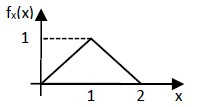
\includegraphics[width=0.3\linewidth]{imagenes/Actividad_3/actividad_3.jpg}
        \caption{Función de densidad.}
        \label{fig:diagrama_3}
    \end{figure}

\subsection*{a) Calcular analíticamente la media, la varianza y la desviación estándar.}


\subsection*{b) Calcular y graficar la función de distribución acumulada.}


\subsection*{c) Calcular \( P(0.75 \leq X \leq 1.75) \).}


\subsection*{d) Realizar un código que permita generar vector de 500 muestras aleatorias y graficar el histograma de esas muestras. Luego calcular la media 
y la varianza.}

	\section{Actividad 4}

\subsection*{Graficar las señales senoidales correspondientes que cumplan las siguientes condiciones:}

\subsection*{a) Señal de amplitud \(A\) aleatoria uniforme, distribuida entre \([8, 40]\).}

    \[
        x(t) = A \cos(2 \pi 10 t)
    \]

\subsection*{b) Señal de fase \(\Theta\) aleatoria uniforme, distribuida entre \([-\pi, \pi]\).}

    \[
        x(t) = 5 \cos(2 \pi 10 t + \theta)
    \]

\subsection*{c) Señal de frecuencia \(f\) aleatoria uniforme, distribuida entre \([0, 20 ]\).}

    \[
        x(t) = 5 \cos(2 \pi f t)
    \]

\subsection*{d) Señal de amplitud, fase y frecuencia aleatoria, distribuidas de igual forma que los
puntos anteriores.}

\subsection*{Además, graficar la auto‐correlación para todos los puntos anteriores. ¿Qué información se obtienen al observar la gráfica de auto‐correlación?.}
	\section{Actividad 5}

\subsection*{En el trabajo práctico anterior se analizó espectralmente una señal compuesta por tres 
sinusoides de frecuencias 50 Hz, 120 Hz y 200 Hz, con diferentes amplitudes y fases 
(constantes).}

\subsection*{a) Graficar la señal total en el dominio del tiempo y en el dominio de la frecuencia 
(mediante la Transformada Rápida de Fourier, FFT).} 

La señal total del práctico anterior es la siguiente:

\[
      \begin{aligned}
            x(t) &= 1.0 \cos\!\bigl(2\pi 50 t\bigr)
                  + 0.5 \cos\!\bigl(2\pi 120 t\bigr)
                  + 0.3 \cos\!\bigl(2\pi 200 t\bigr)
      \end{aligned}
\]

\bigskip
      \begin{figure}[H]
            \centering
            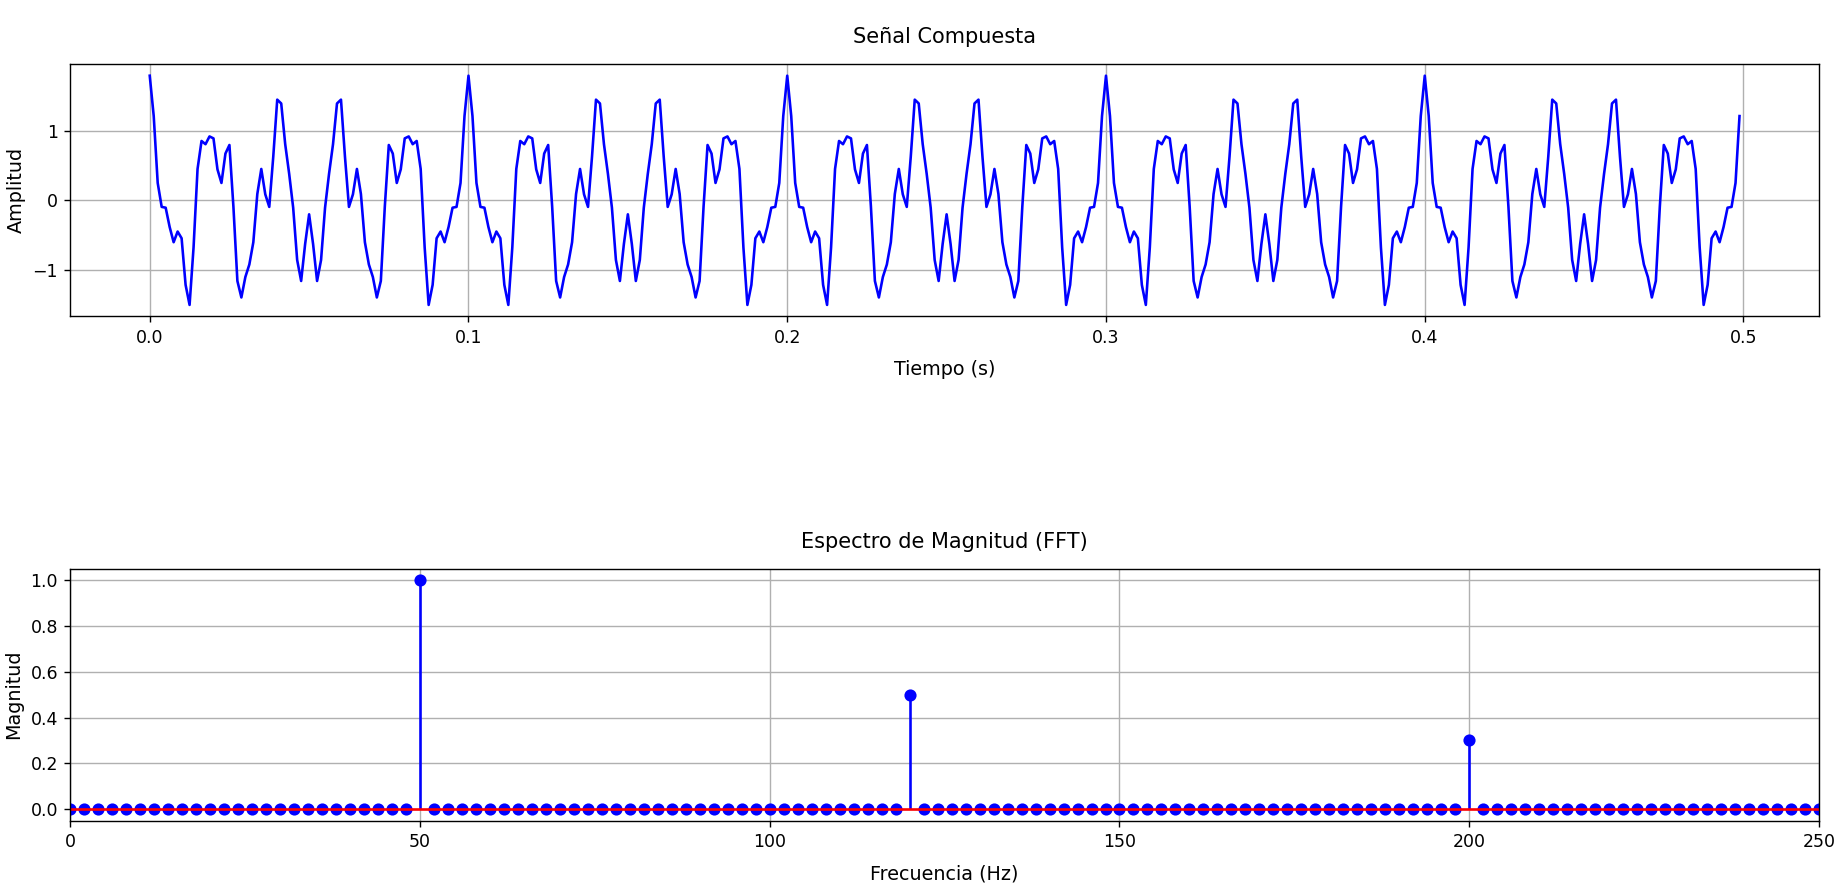
\includegraphics[width=0.8\textwidth]{imagenes/Actividad_5/senalcompuesta.png}
            \caption{Señal total.}
      \end{figure}
\bigskip

\subsection*{b) Incorporar a la señal ruido blanco gaussiano en dos escenarios:}

\begin{itemize}
    \item Ruido bajo: el nivel de ruido no es suficiente para ocultar las componentes sinusoidales.
    \item Ruido alto: el nivel de ruido es suficiente para enmascarar las componentes de la señal.
\end{itemize}

Para cada caso, representar nuevamente la señal tanto en el tiempo como en el espectro de frecuencias y analizar cómo varían la 
visibilidad de las componentes espectrales. \par

\bigskip
      \begin{figure}[H]
            \centering
            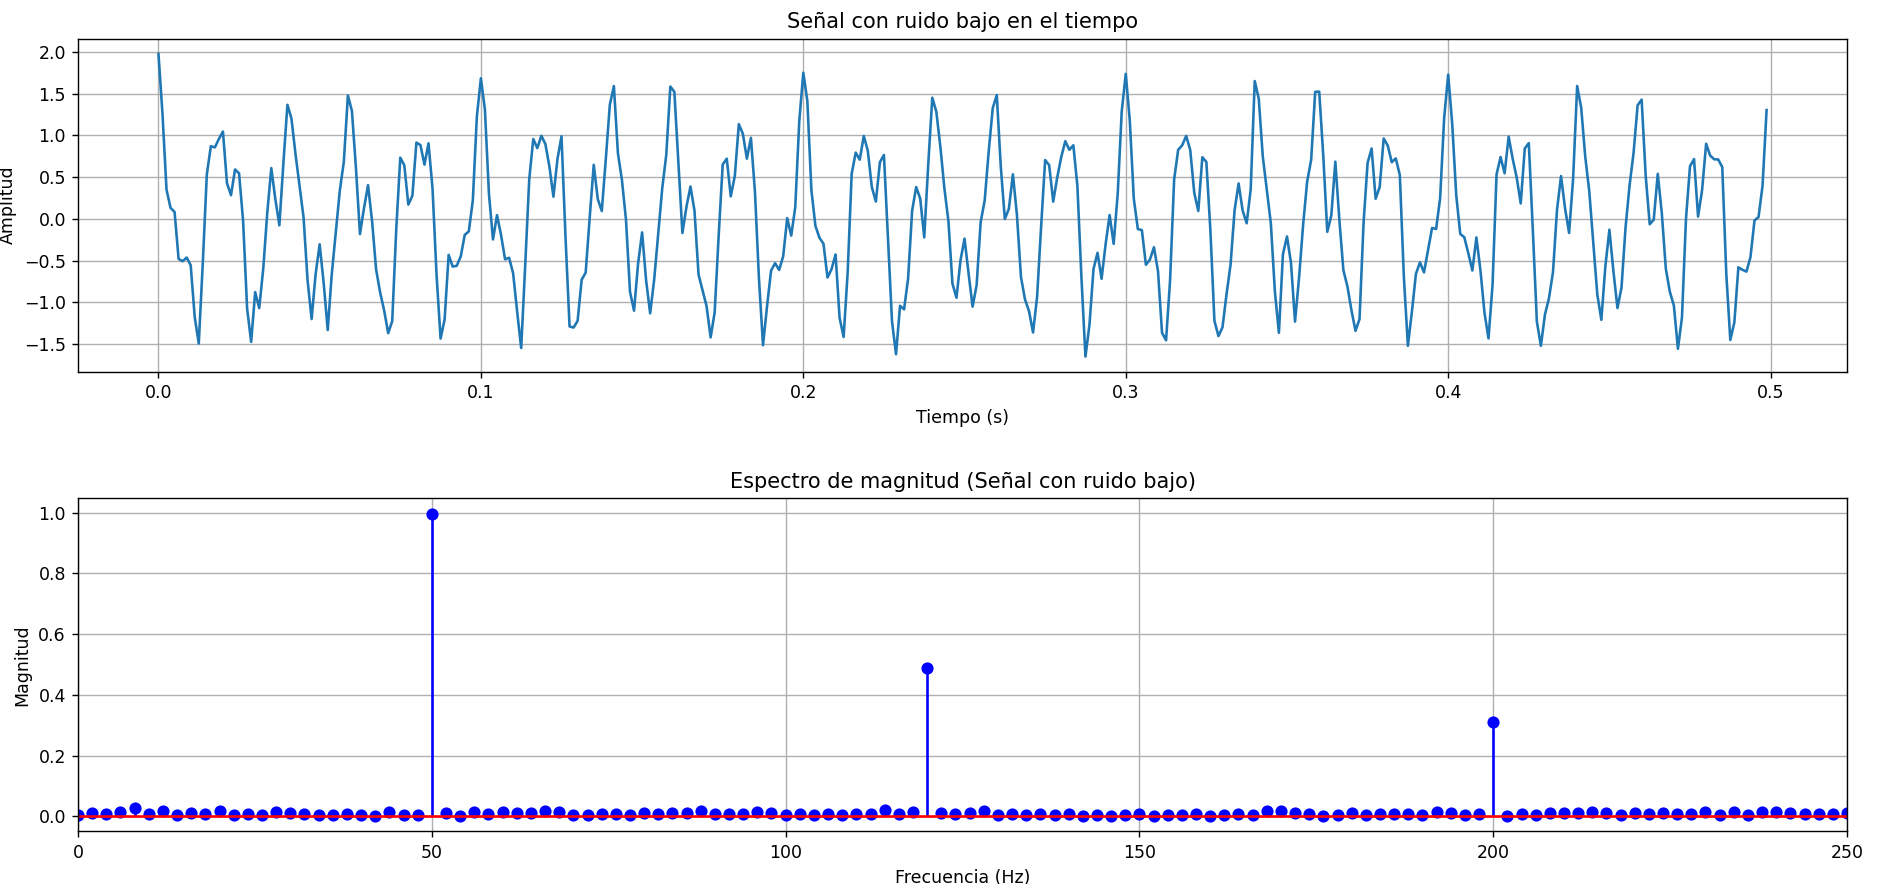
\includegraphics[width=0.8\textwidth]{imagenes/Actividad_5/senalconruidobajo.png}
            \caption{Señal con rudio blanco gaussiano bajo.}
      \end{figure}
\bigskip

\bigskip
      \begin{figure}[H]
            \centering
            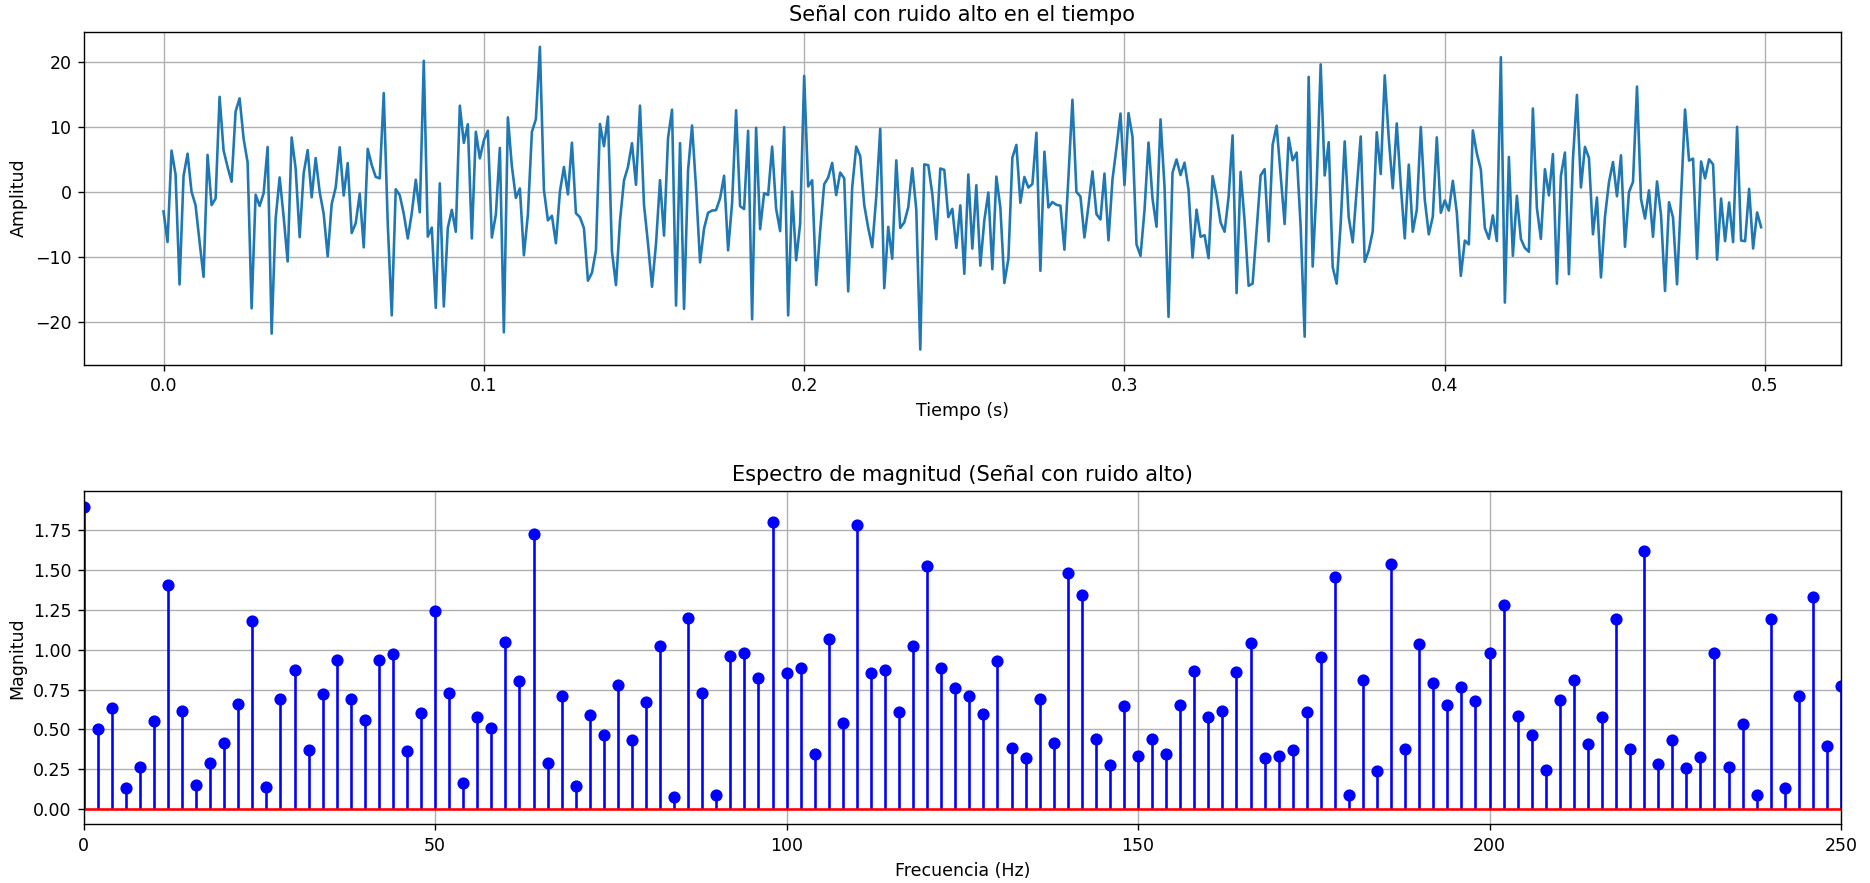
\includegraphics[width=0.8\textwidth]{imagenes/Actividad_5/senalconruidoalto.png}
            \caption{Señal con rudio blanco gaussiano alto.}
      \end{figure}
\bigskip


En las Figuras 5 se observan la gráfica de la señal total con ruido bajo agregado.
\bigskip

Al comparar la señal total con las versiones con ruido, se logra verificar que en el dominio del tiempo la misma no posee ruido, 
presenta una forma suave y definida, mientras que con ruido bajo aparecen pequeñas variaciones sin perder la forma general. Mientras
que con ruido alto la forma original se pierde debido a las variaciones aleatorias. En el dominio de la frecuencia, la señal total sin 
ruido, muestra tres picos en 50 Hz, 120 Hz y 200 Hz, con las frecuencias fuera de las mencionadas en casi cero. Al añadir ruido bajo 
los picos siguen visibles aunque surge un nivel de ruido en todo el espectro (piso de ruido).En cambio, con ruido alto ese piso 
aumenta y los picos se atenúan o se confunden con el ruido. Esto quiere decir que un ruido creciente degrada la forma temporal y 
espectral, dificultando identificar las componentes de la señal original.\par

\bigskip

Por último, se calcula la relación señal-ruido (SNR) para la señal compuesta con amplitudes $A_1=1.0$, $A_2=0.5$ y $A_3=0.3$. 
La potencia media de la señal compuesta se calcula como $A_i^2/2$.

El ruido añadido es blanco y gaussiano con media cero y desviación estándar $\sigma$, por lo que su potencia es $\sigma^2$. 
La relación señal-ruido en decibelios se calcula mediante 
$\text{SNR}_{\mathrm{dB}}=10\log_{10}\!\bigl(P_{\text{señal}}/P_{\text{ruido}}\bigr)$. 
Para el caso de ruido bajo se obtiene un SNR elevado, lo que implica que las componentes espectrales son claramente visibles, 
mientras que para el caso de ruido alto la potencia de ruido domina a la de la señal y se difuculta identificar las componentes de 
la señal total.
\bigskip

\noindent \[
      P_{\text{señal}} = 
      \frac{A_1^2}{2}+\frac{A_2^2}{2}+\frac{A_3^2}{2}=
      \frac{1^2+0.5^2+0.3^2}{2}=
      \frac{1+0.25+0.09}{2}=0.67
\]

\noindent \[
      P_{\text{ruidobajo}}=\sigma_{\text{bajo}}^2=0.1^2=0.01
      \quad\text{y}\quad
      P_{\text{ruidoalto}}=\sigma_{\text{alto}}^2=8^2=64
\]

\noindent \[
      \text{SNR}_{\text{bajo}}=
      10\log_{10}\!\left(\frac{0.67}{0.01}\right)=10\log_{10}(67)=18.3~\text{dB}
\]

\noindent \[
      \text{SNR}_{\text{alto}}=
      10\log_{10}\!\left(\frac{0.67}{64}\right)=10\log_{10}(0.01047)=-19.8~\text{dB}
\]

	\section{Actividad 6}

\subsection*{Considerar el diagrama ilustrado en la Fig. \ref{sistema}. Se tiene la primera etapa con un filtro pasa banda, al cual
ingresa ruido blanco Gaussiano, de media cero y densidad espectral de potencia N0/2. Seguido a ello se tiene un modulador producto y 
finalmente un filtro pasa bajo. Las respuestas en frecuencia de ambos filtros pueden observarse en las Fig. \ref{pasabanda} y
Fig. \ref{pasabajo}.}


	\begin{figure}[H]
		\centering
		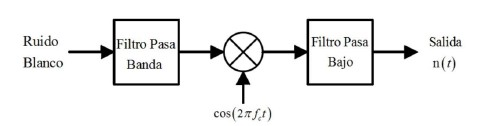
\includegraphics[width=12cm]{imagenes/Actividad_6/act_6_sistema.jpg}
		\caption{Esquema de la actividad 6.}
		\label{sistema}
	\end{figure}

	\begin{figure}[H]
		\centering
		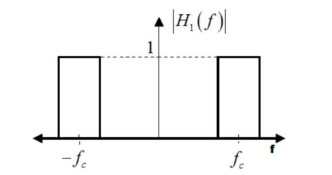
\includegraphics[width=6cm]{imagenes/Actividad_6/act6_pasabanda.jpg}
		\caption{Respuestas en frecuencia del filtro pasa banda.}
		\label{pasabanda}
	\end{figure}

	\begin{figure}[H]
		\centering
		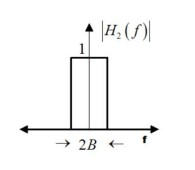
\includegraphics[width=4cm]{imagenes/Actividad_6/act_6_pbajos.jpg}
		\caption{Respuestas en frecuencia del filtro pasa bajo.}
		\label{pasabajo}
	\end{figure}



\subsection*{a) Calcular la densidad espectral de potencia y la función autocorrelación de $n(t)$. Graficar que se obtiene a la salida 
de cada filtro y del modulador producto (no debe usar el programa).} \par

	La densidad espectral de potencia del ruido $n(t)$ en la salida del filtro pasabanda es:
		\[
			S_{NP_{Banda}}(f) =
			\begin{cases}
			\dfrac{N_0}{2} & -f_c - B < f < -f_c + B \\[6pt]
			\dfrac{N_0}{2} & f_c - B < f < f_c + B \\[6pt]
			0 & \text{o.c.}
			\end{cases}
		\]

	El gráfico de la densidad espectral de potencia a la salida del filtro pasabanda se observa en la Fig. \ref{fig:6pasabanda}.

		\begin{figure}[H]
			\centering
			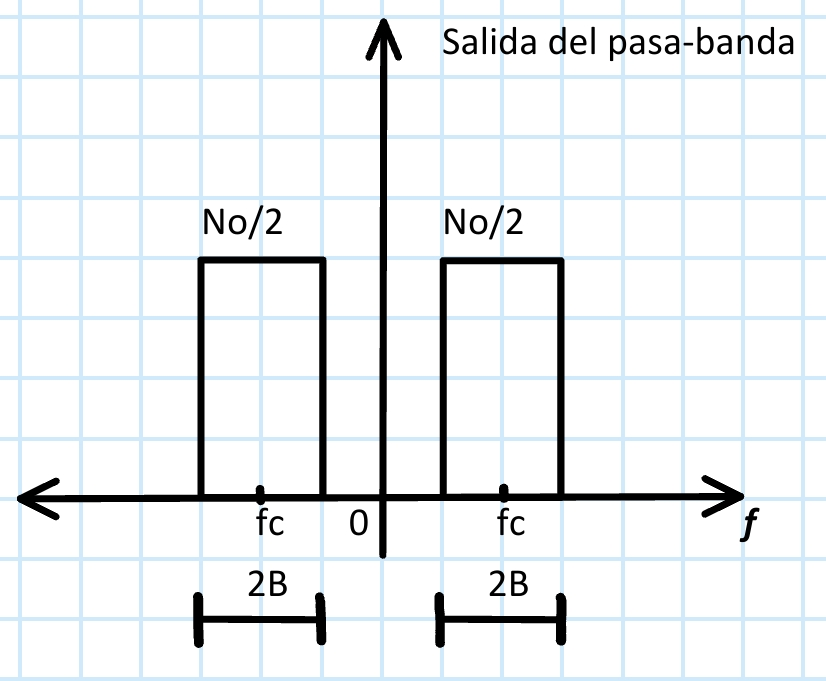
\includegraphics[width=7cm]{imagenes/Actividad_6/actividad6_pasabanda.jpg}
			\caption{Densidad espectral de potencia del filtro pasabanda.}
			\label{fig:6pasabanda}
		\end{figure}


	Luego, la salida del filtro pasabanda se multiplica por la señal portadora $\cos(2 \pi f_c t)$, donde la transformada de 
	Fourier de dicha portadora es:
		\[
			\cos(2 \pi f_c t) = \tfrac{1}{2} \left[ \delta(f - f_c) + \delta(f + f_c) \right]
		\]
	
	Al multiplicar en el dominio del tiempo, se realiza una convolución en el dominio de la frecuencia, por lo que la densidad espectral de potencia en la 
	salida del modulador producto es:

		\[
			S_{N_{Modulador}}(f) =
			\begin{cases}
			\dfrac{N_0}{4} & -2f_c - B < f < -2f_c + B \\[6pt]
			\dfrac{N_0}{2} & -B < f < B \\[6pt]
			\dfrac{N_0}{4} & 2f_c - B < f < 2f_c + B \\[6pt]
			0 & \text{o.c.}
			\end{cases}
		\]
	
	El gráfico de la densidad espectral de potencia a la salida del modulador producto se observa en la Fig. \ref{fig:6modulador}.


		\begin{figure}[H]
			\centering
			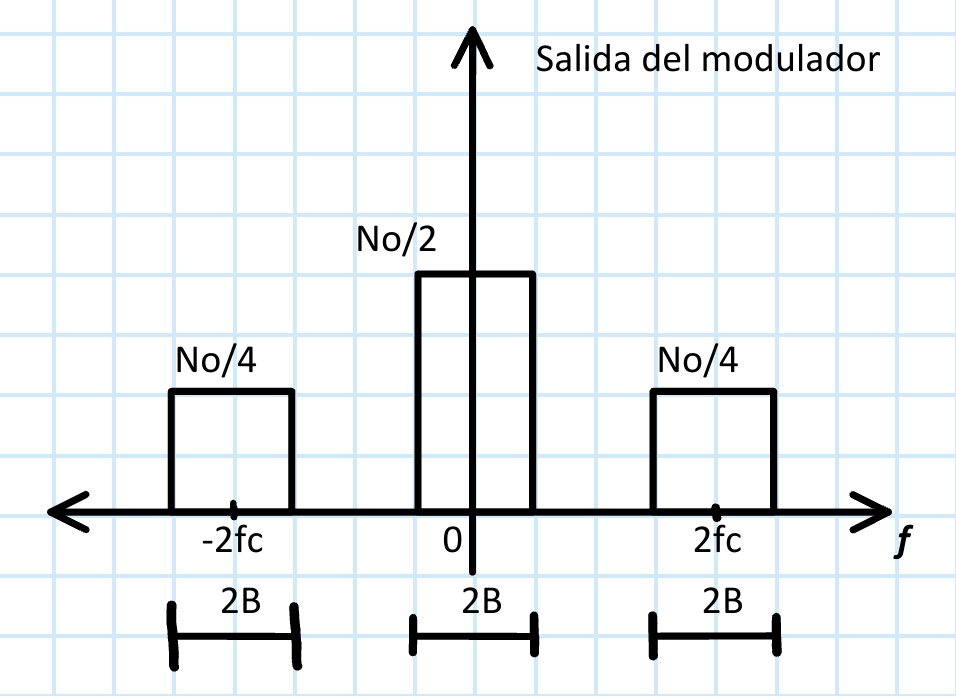
\includegraphics[width=7cm]{imagenes/Actividad_6/actividad6_modulador.jpg}
			\caption{Densidad espectral salida modulador.}
			\label{fig:6modulador}
		\end{figure}



	Finalmente, la salida del modulador producto ingresa al filtro pasabajo, por lo que la densidad espectral de potencia en 
	la salida del filtro pasabajo es:
		\[
				S_{N_{PasaBajo}}(f) =
				\begin{cases}
				\dfrac{N_0}{2} & -B < f < B \\[6pt]
				0 & \text{o.c.}
				\end{cases}
		\]

	El gráfico de la densidad espectral de potencia a la salida del filtro pasabajo se observa en la Fig. \ref{fig:6pasabajo}.
    
		\begin{figure}[H]
			\centering
			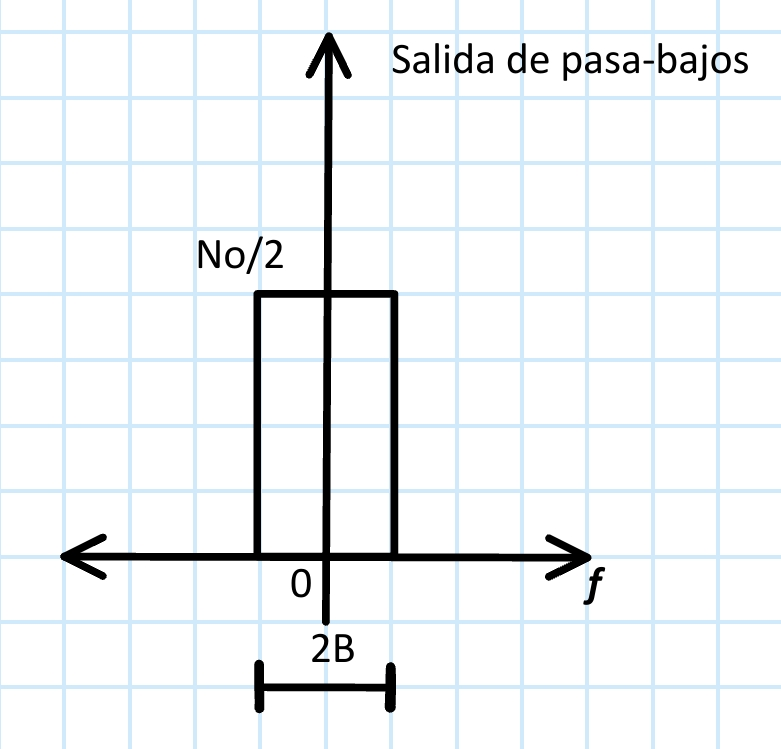
\includegraphics[width=7cm]{imagenes/Actividad_6/actividad6_pasabajo.jpg}
			\caption{Densidad espectral salida filtro pasa bajo.}
			\label{fig:6pasabajo}
		\end{figure}

	La función de autocorrelación se obtiene a partir de la transformada inversa de la densidad espectral de potencia, es 
	decir:
		\[
			R_{n(t)}(\tau) = \int_{-\infty}^{\infty} S_{N_{PasaBajo}}(f) e^{j 2 \pi f \tau} df
		\]
	Reemplazando la densidad espectral de potencia obtenida en la salida del filtro pasabajo, se tiene:
		\[
			R_{n(t)}(\tau) = \int_{-B}^{B} \dfrac{N_0}{2} e^{j 2 \pi f \tau} df
		\]
	Resolviendo la integral se obtiene:
		\[
			R_{n(t)}(\tau) = N_0 B \, \text{sinc}(2 B \tau)
		\]
	

\subsection*{b) Calcular la media y la varianza de n(t).} \par

	El ruido blanco gaussiano de entrada tiene media cero, y los filtros lineales e invariantes en el tiempo (filtro pasa banda 
	y filtro pasa bajo) no alteran la media si la entrada tiene media cero. Esto se deduce de la siguiene ecuación:
	
		\[
			\mu_Y = \mu_X \int_{-\infty}^{\infty} h(\tau_1)\, d\tau_1 = \mu_X H(0)
		\]

	Por lo tanto, como la media $\mu_x$ dell ruido en la entrada es cero , entonces la media de $n(t)$ es:
		\[
			\mu_{n(t)} = \mu_x H(0) = 0 \cdot 1 = 0
		\]
	
	Para calcular la varianza se utiliza la siguiente ecuación:

		\[
		\sigma_x^2 = E[x^2] - \mu_x^2
		\]

	Por propiedad de autocorrelación se tiene que \(R_x(0) = E[x^2]\), reemplazando se obtiene lo siguiente:

		\[
		\sigma_x^2 = R_x(0) - 0 = N_0 B \, \text{sinc}(0)
		\]

		\[
		\sigma_x^2 = N_0 B
		\]


\subsection*{c) ¿Cuál es la tasa a la cual $n(t)$ puede ser muestreada, de manera tal de que las muestras resultantes sean no
 correlacionadas?} \par

	Para que las muestras resultantes sean no correlacionadas se busca que la función de autocorrelación sea igual a 0. Entonces,
	teniendo en cuenta la Ecuación 8, esta función da 0 cuando el valor dentro del seno cardinal es un entero
		

		\[
			2B\tau = k, \quad k \in \mathbb{Z}
		\]

	Entonces

		\[
			\tau = \frac{k}{2B}
		\]

		\[
			f_{\text{muestreo}} = \frac{2B}{k}
		\]

	Por lo tanto, la tasa de \(n(t)\) debe ser al menos \(2B\) muestras por segundo para que las muestras 
	resultantes sean no correlacionadas.

	\section{Actividad 7}

\subsection*{En la Fig. \ref{fig:diagrama} podrá observar el diagrama en bloques simplificado de un receptor de televisión satelital 
(similar a los que se encuentran en centros de distribución CATVCommunity Antenna Television). La temperatura de ruido antena-línea 
de alimentación es 50 K. Calcular la temperatura equivalente de ruido del sistema.}

    \begin{figure}[H]
            \centering
            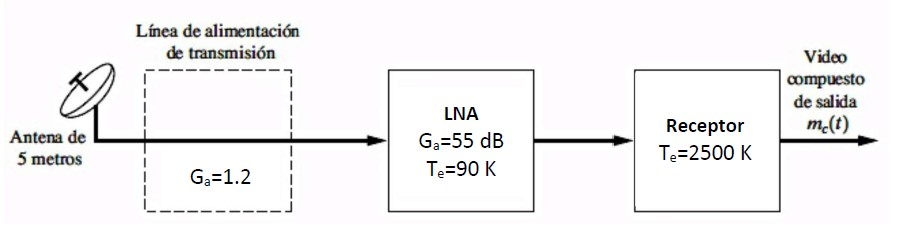
\includegraphics[width=0.8\linewidth]{imagenes/Actividad_7/actividad_7.jpg}
            \caption{Diagrama en bloques.}
            \label{fig:diagrama}
    \end{figure}

    Utilizando la fórmula de Friis, la cual permite expresar la temperatura de ruido equivalente de un sistema compuesto por varias etapas en función de las 
    temperaturas de ruido y ganancias de cada etapa, se tiene que:
        
        \[
            T_{eq} = T_1 + \frac{T_2}{G_1} + \frac{T_3}{G_1 G_2} + \cdots           
        \]
    
    Para proceder con los calculos se necesita convertir las ganancias de dB a unidades lineales utilizando la fórmula:
    
        \[
            G_{linear} = 10^{\frac{G_{dB}}{10}}
        \]
    
    Al realizar las conversiones requeridas se obtienen los siguientes valores:
        \begin{itemize}
            \item $G_1 = 1,2$
            \item $G_2 = 316227,766$
        \end{itemize}

    Ahora, se sustituyen los valores conocidos en la fórmula de Friis:
        \[
            T_{eq} = 50 k + \frac{900 k }{1,2} + \frac{2500 k }{1,2 \times 316227,766} = 125,0088 k
        \]

    Por lo tanto, la temperatura equivalente de ruido del sistema es igual a $125,0088 K$.

	\section{Actividad 8}

\subsection*{En un determinado circuito se tienen tres amplificadores conectados en cascada, tal
como se puede observar en la Fig. }

    \begin{figure}[H]
        \centering
        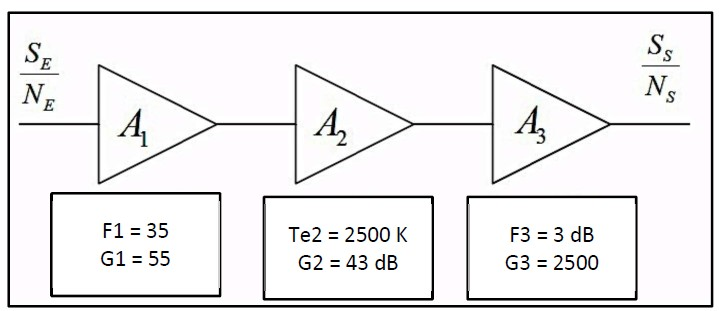
\includegraphics[width=0.8\linewidth]{imagenes/Actividad_8/actividad_8.jpg}
        \caption{Circuito en cascada.}
        \label{fig:diagrama_8}
    \end{figure}

\subsection*{Calcular:}

\subsection*{a) La figura de ruido total, suponiendo la temperatura ambiente T = 290 K.}

\subsection*{b) La temperatura equivalente de ruido total.}

\subsection*{c) Intercambiar los amplificadores A1 y A3. Calcular nuevamente la figura de ruido total, y explicar que sucede.}

\subsection*{d) Suponer que ingresa a la cascada de amplificadores una señal con una potencia de 20x10-9 W. Calcular la relación señal ruido 
tanto en la entrada, como en la salida de dicha cascada, considerando $\Delta f = 150 kHz$.}
    

%\printbibliography[heading=bibintoc] % Agrega el título "Referencias" al índice automáticamente
    
\end{document}
